% \begin{table}[ht!]
\centering
\resizebox{0.95\linewidth}{!}{
\begin{tabular}{l|lll}
\hline
\hline
    Method (split)            & AMOTA $\uparrow$  & Recall $\uparrow$ & MOTA $\uparrow$   \\
    \hline
    AB3DMOT + CP (test) & 0.387             & 0.506             & 0.284             \\
    \hline
    Best Hyper-parameters (test)       & \textbf{0.402}    & \textbf{0.511}    & \textbf{0.320        }     \\
    \hline
    $w_{iou} = 1.4 $ (validation)   & 0.403             & 0.540             & 0.322               \\
    $w_{center} = 0.9$ (validation) & 0.417             & 0.514             & 0.332             \\
    $w_{embedd} = 0.4$ (validation) & 0.418             & 0.558             & 0.332             \\
    $\tau_{det} = 0.4$ (validation) & 0.397             & 0.567            & 0.326             \\
\hline
\hline
\end{tabular}
}
\caption{\textbf{Optimized Matching and Detection Confidence.} Parameters were optimized on the nuScenes \cite{caesar2020nuscenes} validation set. On the test split our best setting with $w_{iou} = 1.4$, $w_{center} = 0.9$, $w_{embbed} = 0.4$, $\tau_{det} = 0.4$ surpasses the performance of AB3DMOT \cite{weng2020AB3DMOT}, the only baseline not trained on the dataset. Results for other baselines are given in Tab. \ref{tab:nuScenes_results}. \todo{rewrite} }\label{tab:matching_ablations}
\vspace{-12pt}
\end{table}
% \begin{table}[t]
\centering
\resizebox{0.9\linewidth}{!}{
\begin{tabular}{l|lll}
    \hline
    \hline
    Method & AMOTA $\uparrow$ & Recall $\uparrow$  & MOTA$\uparrow$  \\
    \hline
    No Schedule & 0.102 & 0.224 & 0.110  \\
    \hline
    $\mathcal{L}_{RGB}$ - Eq.~\ref{eq:loss_mse} & N/A  & N/A & N/A  \\
    $\mathcal{L}_{perceptual}$ - Eq.~\ref{eq:loss_lpips} & 0.100 & 0.251 & 0.101 \\
    $\mathcal{L}_{IR}$ - Eq.\ref{eq:loss_mse_lpips}  & 0.103 & 0.236   & 0.112 \\
    $\mathcal{L}_{IR}$ \& $\mathcal{L}_{embed}$ - Eq.\ref{eq:regularize}  & \textbf{0.112} & \textbf{0.264 } & \textbf{0.113} \\
\hline
\hline
\end{tabular}
}
\caption{\todo{(a) Make split figure} \textbf{Ablation Experiments on Optimization Schedule and Loss Components.} Ablations were run on a small subset of the nuScenes~\cite{caesar2020nuscenes} validation set.  $\mathcal{L}_{RGB}$ fails due to the optimizer fitting objects to the background instead, increasing the size of each object resulting in out of memory.}
\label{tab:optim_ablations}
\end{table}

\begin{table}[t]
% 1. Table
\caption{\textbf{Ablation Experiments}}
\vspace*{-18pt}
\begin{subtable}[t]{0.485\linewidth}
\centering
\caption{\textbf{Optimization Schedule and Loss Components.} Ablations were run on a small subset of the nuScenes~\cite{caesar2020nuscenes} validation set.  $\mathcal{L}_{RGB}$ fails due to the optimizer fitting objects to the background instead, increasing the size of each object resulting in out of memory.}
% \vspace*{-8pt}
\resizebox{0.98\textwidth}{!}{
\begin{tabular}{l|lll}
    \hline
    \hline
    Method & AMOTA $\uparrow$ & Recall $\uparrow$  & MOTA$\uparrow$  \\
    \hline
    $\mathcal{L}_{IR}$ \& $\mathcal{L}_{embed}$ - Eq.\ref{eq:regularize}  & \textbf{0.112} & \textbf{0.264 } & \textbf{0.113} \\
    $\mathcal{L}_{IR}$ - Eq.\ref{eq:loss_mse_lpips}  & 0.103 & 0.236   & 0.112 \\
    $\mathcal{L}_{perceptual}$ - Eq.~\ref{eq:loss_lpips} & 0.100 & 0.251 & 0.101 \\
    $\mathcal{L}_{RGB}$ - Eq.~\ref{eq:loss_mse} & N/A  & N/A & N/A  \\
    \hline
    \underline{No Schedule} & 0.102 & 0.224 & 0.110  \\
\hline
\hline
\end{tabular}
}
\label{tab:optim_ablations}
\end{subtable}
\hfill
% 2. Table
\begin{subtable}[t]{0.485\linewidth}
\centering
\caption{\textbf{Effect of Optimization Schedule.} (a) observed image, (b) optimized generations using the proposed schedule in Sec.~\ref{sec:method}, (c) optimized generations using no schedule. This supports the quantitative to the left.}
\vspace*{-8pt}
\renewcommand{\arraystretch}{0.4}
\centering
\resizebox{1\columnwidth}{!}{
\begin{tabular}{@{}c@{\hskip .1cm}c@{\hskip .1cm}c@{}}

    \multicolumn{1}{c}{(a) Input Frame} &
    \multicolumn{1}{c}{(b) Full (ours)} & 
    \multicolumn{1}{c}{(c) \underline{No Schedule}} \\
    
    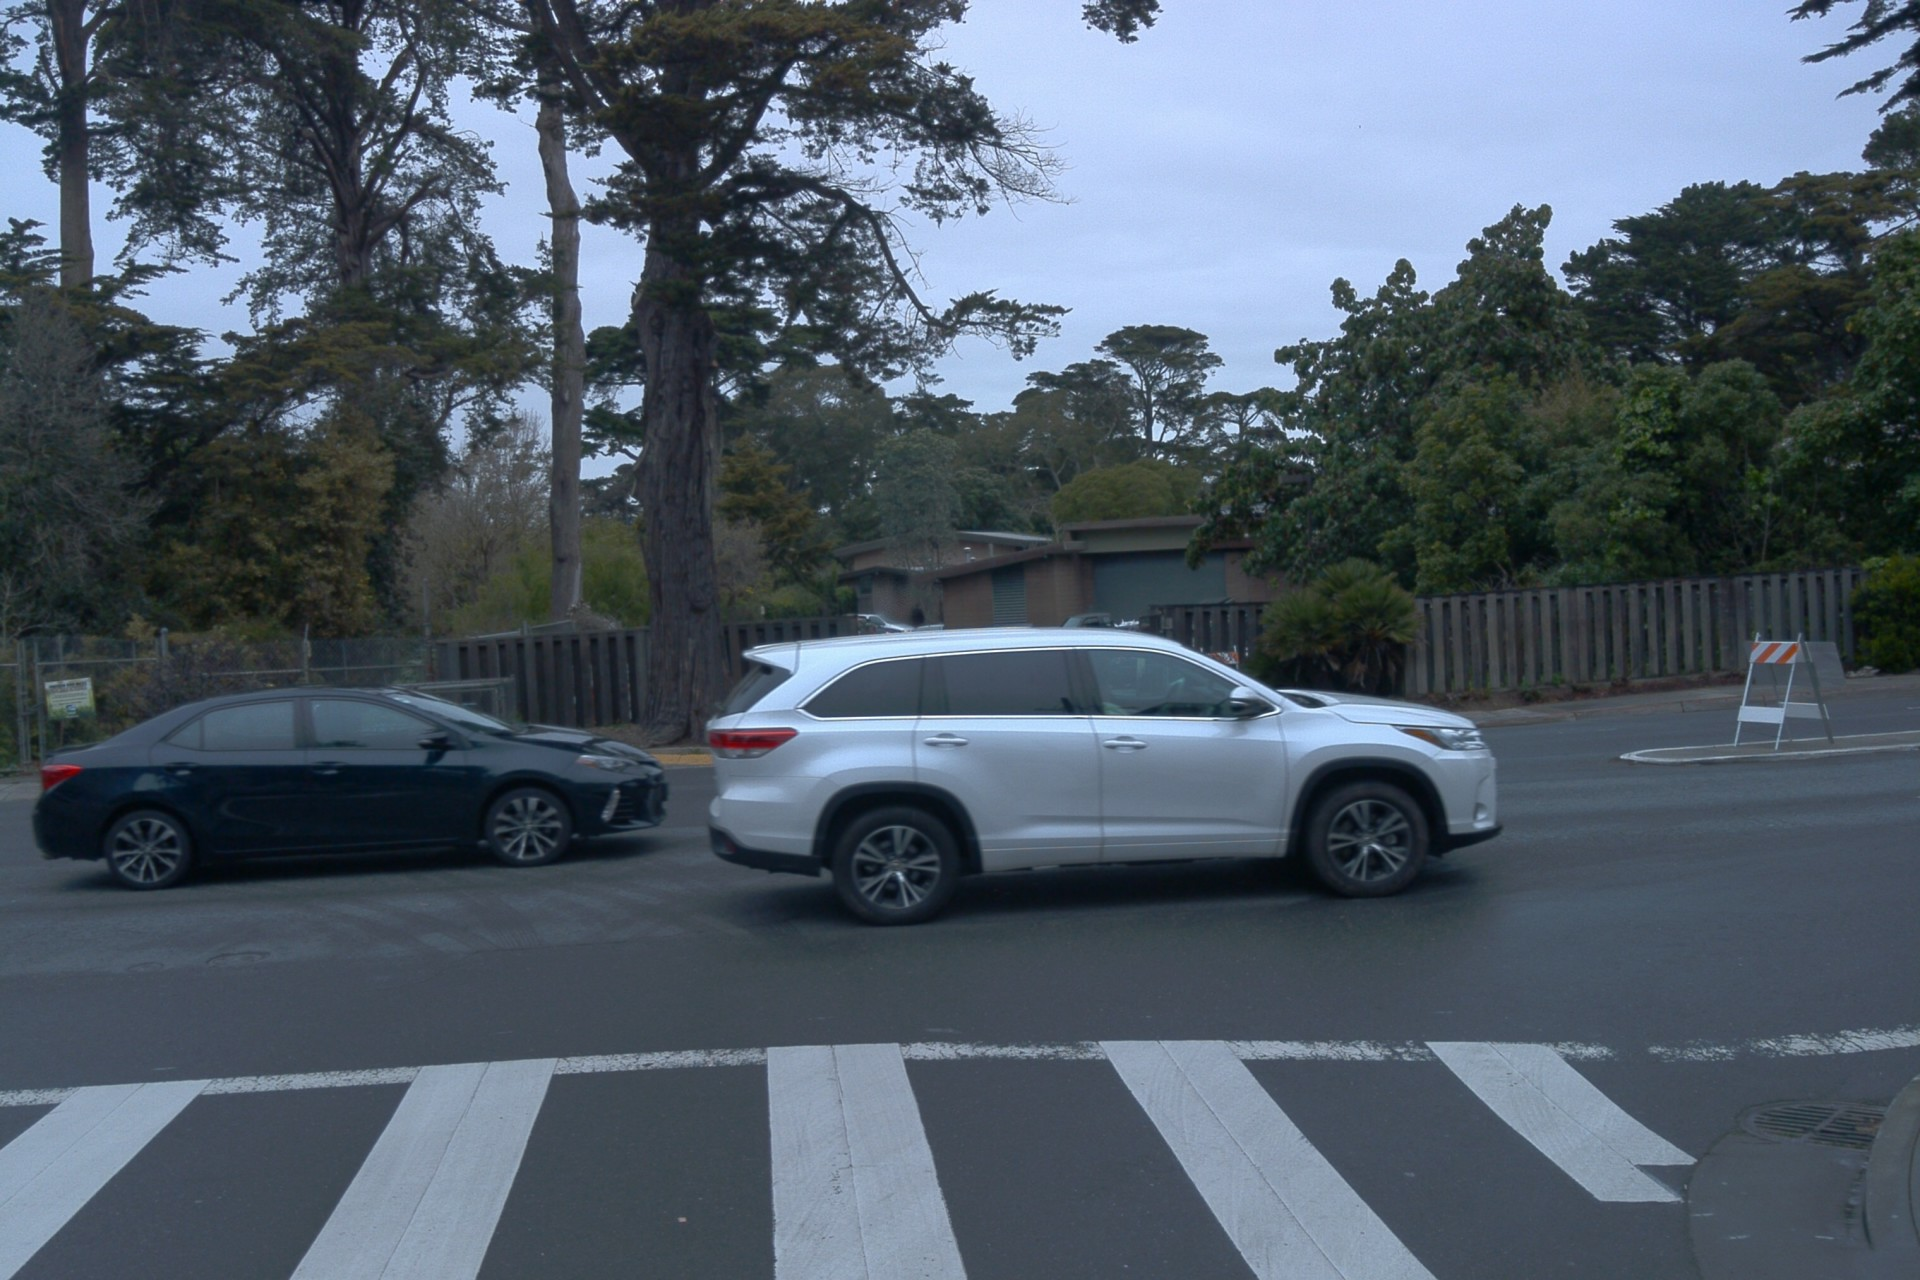
\includegraphics[width=.5\columnwidth, trim={0cm 0cm 0cm 0cm},clip]{fig/rebuttal_optimization/gt/11_102_gt.png}&
    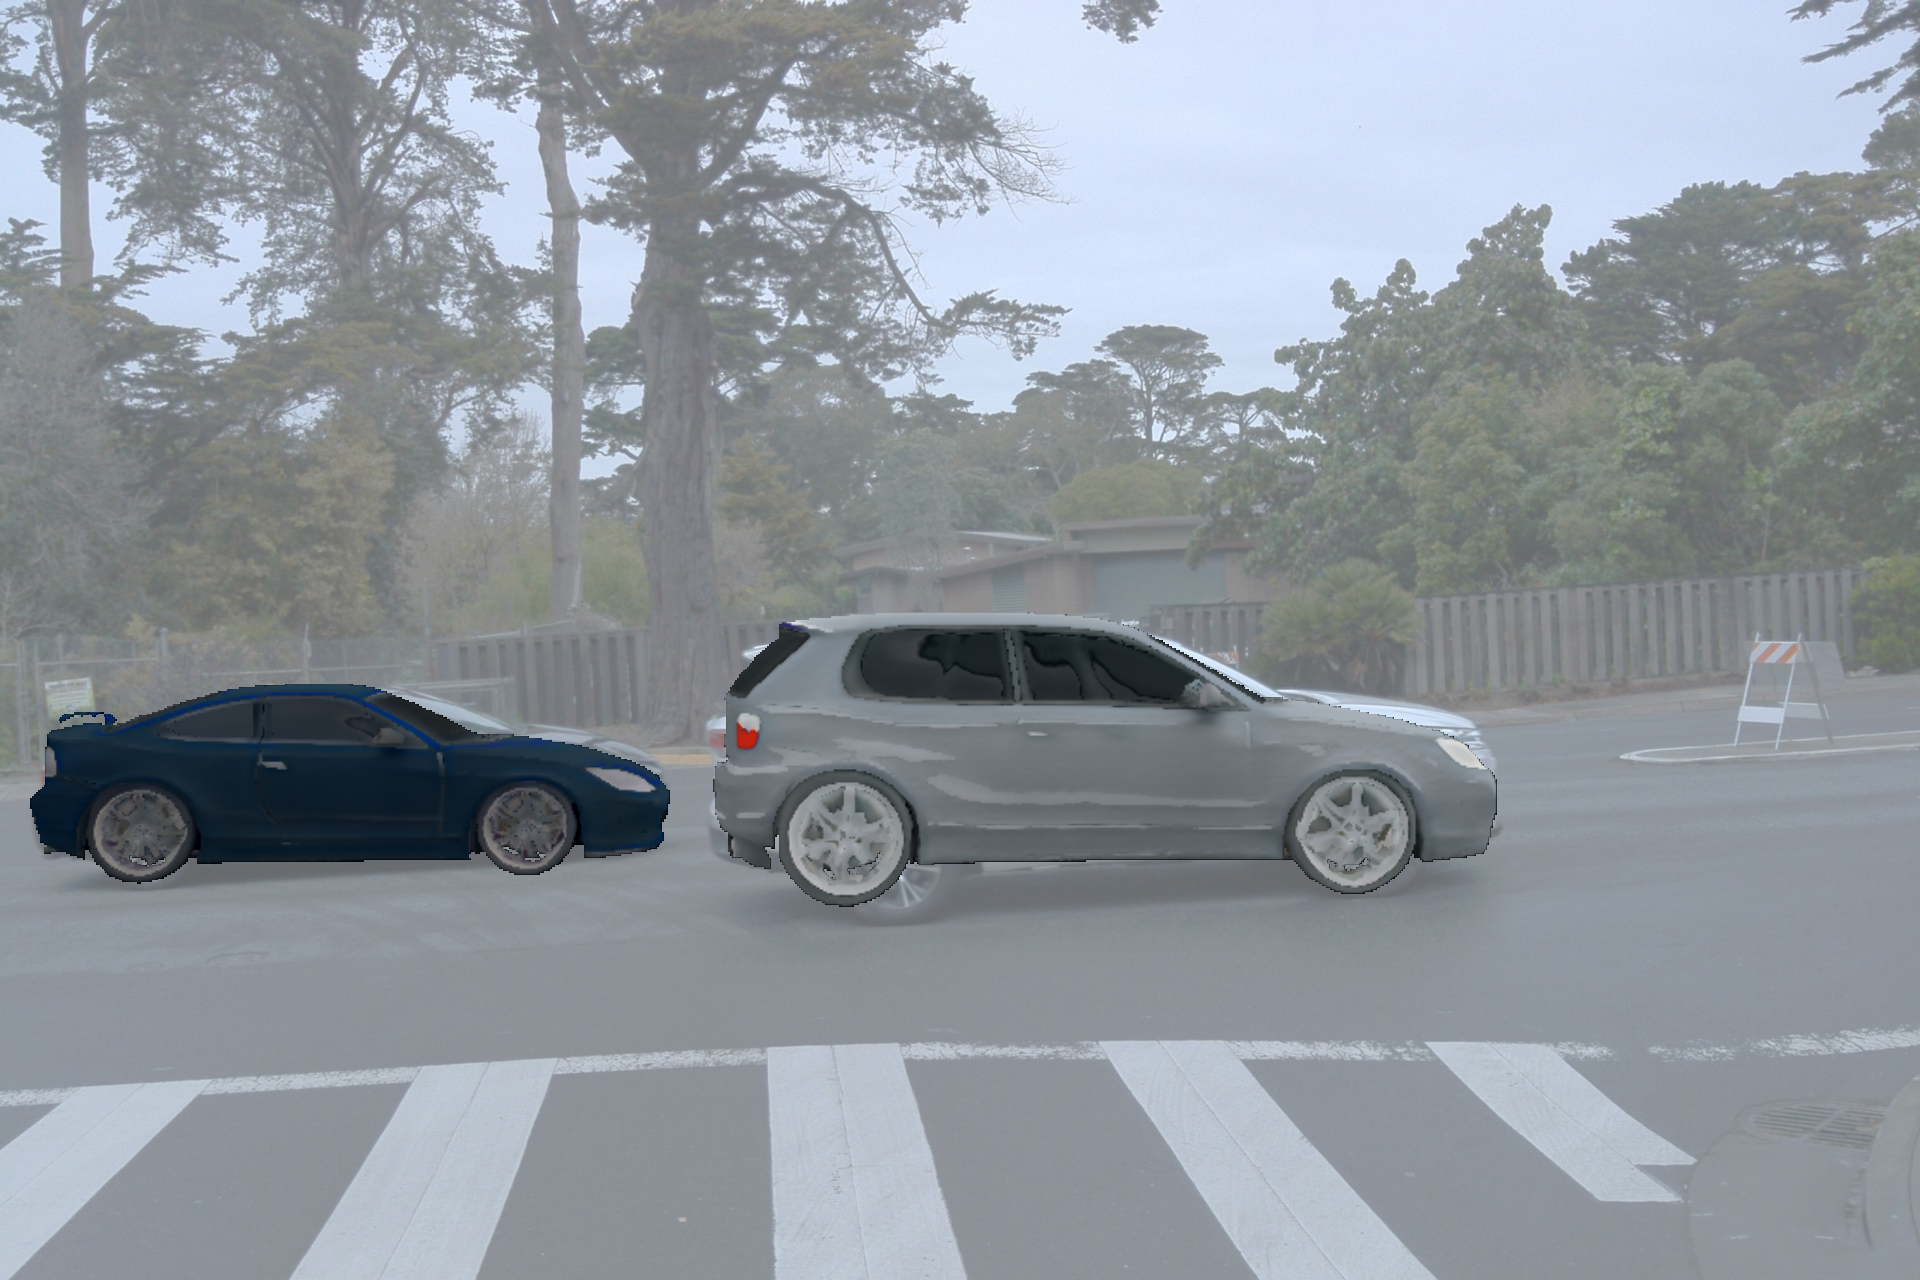
\includegraphics[width=.5\columnwidth, trim={0cm 0cm 0cm 0cm},clip]{fig/rebuttal_optimization/sched/11_102_sched.png}&
    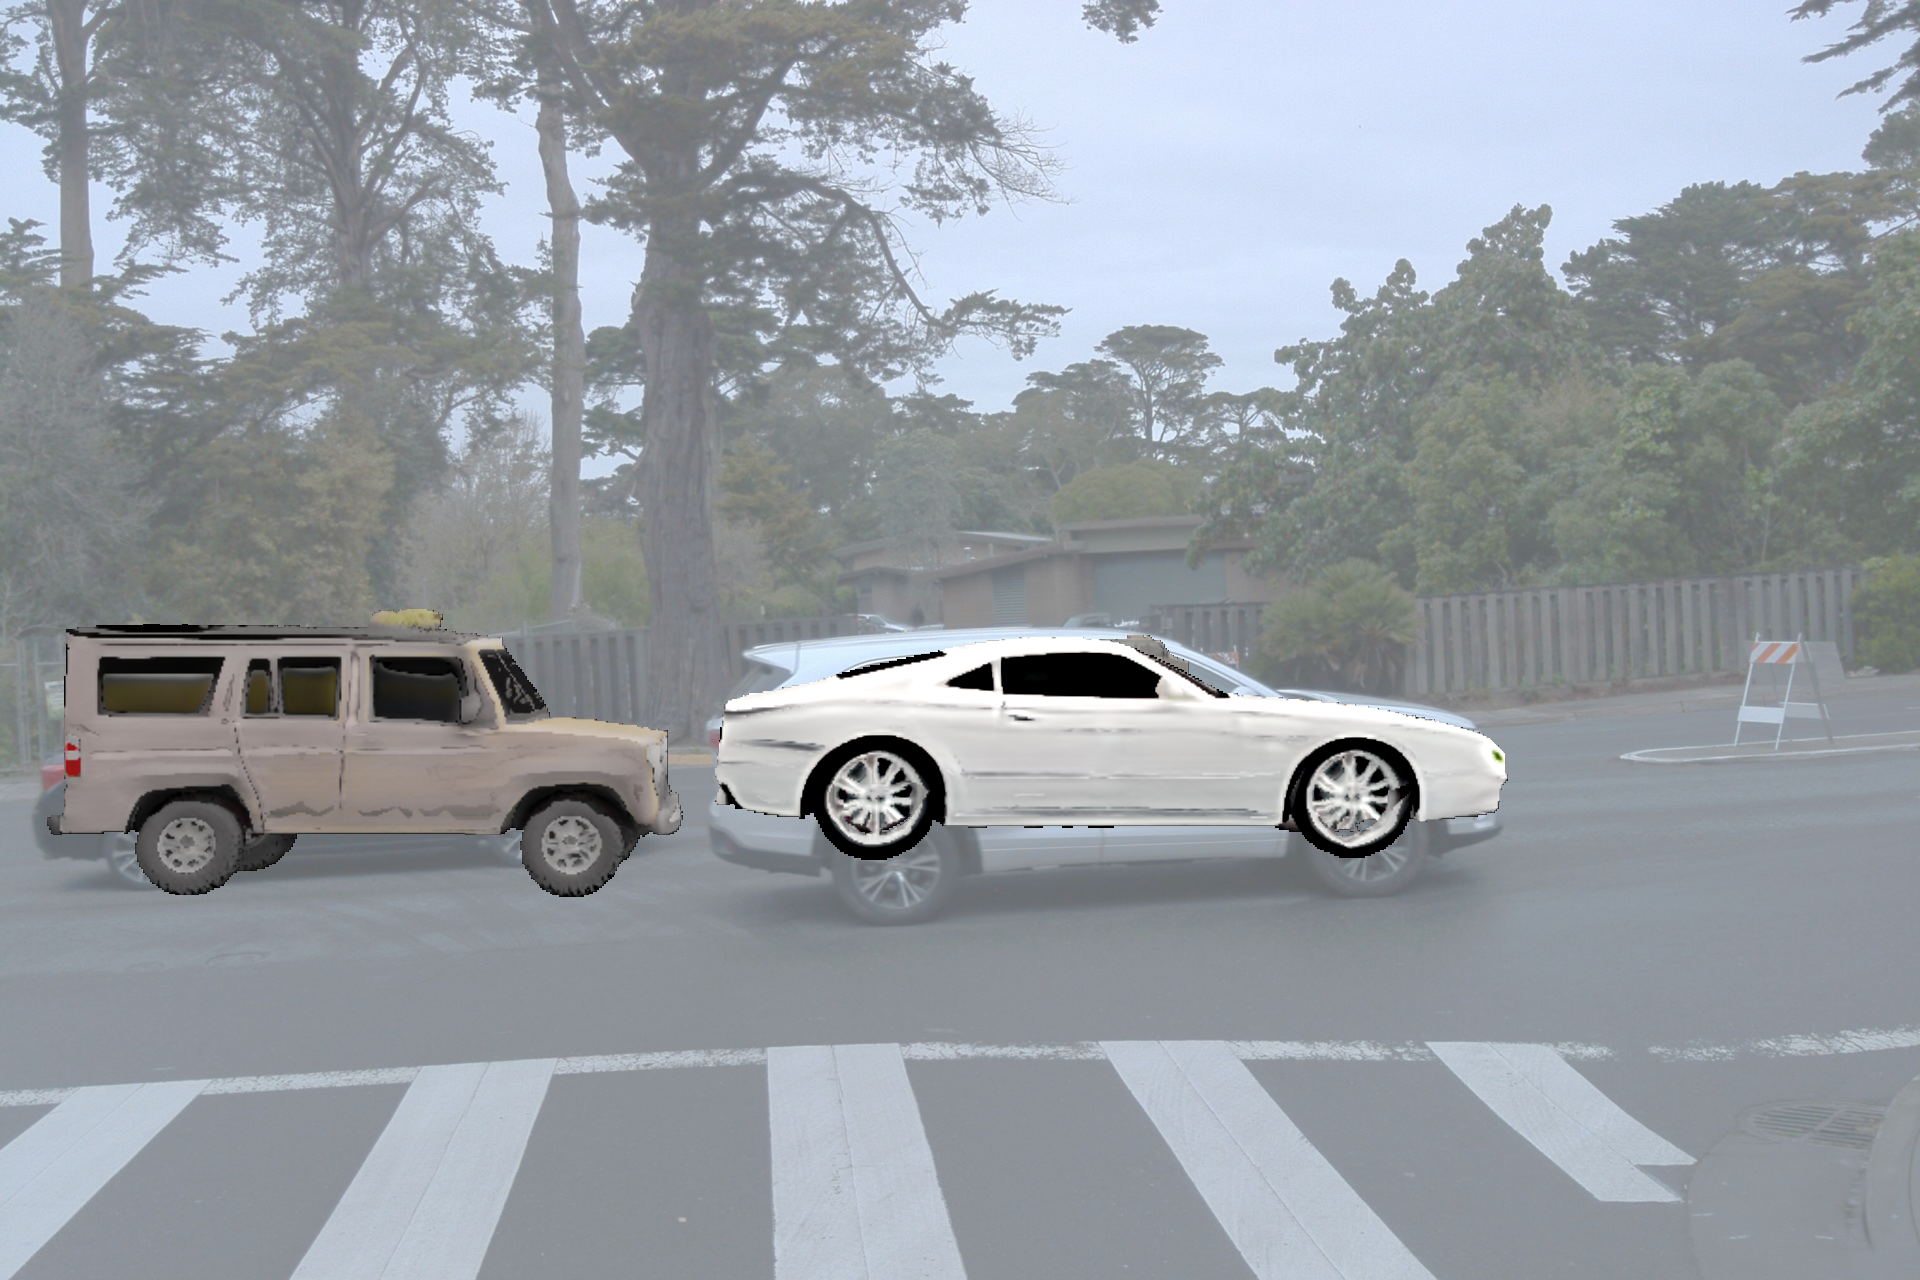
\includegraphics[width=.5\columnwidth, trim={0cm 0cm 0cm 0cm},clip]{fig/rebuttal_optimization/no_sched/11_102_no_sched.png} \\
    
    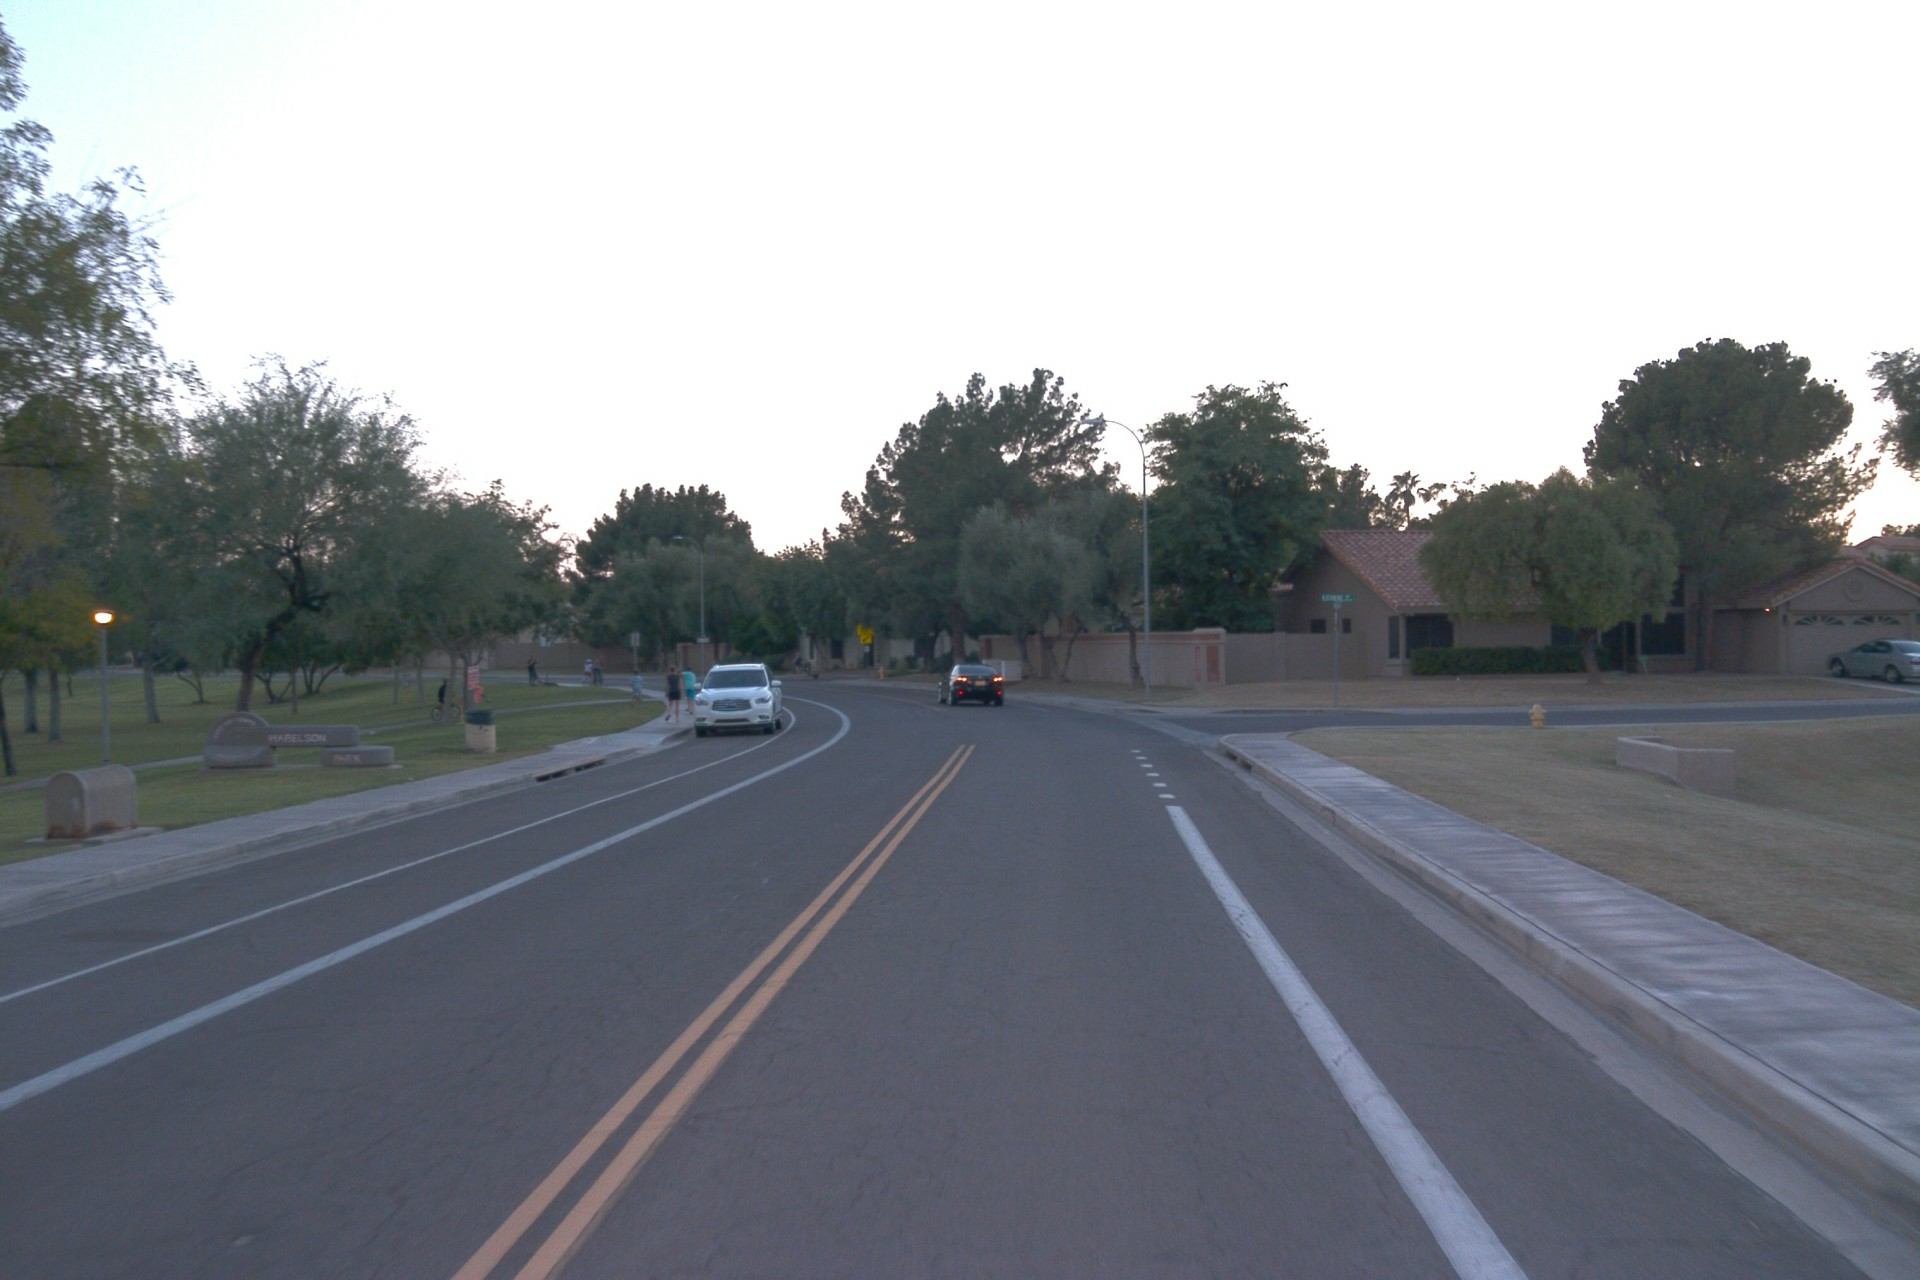
\includegraphics[width=.5\columnwidth, trim={22cm 16.68cm 30cm 18cm},clip]{fig/rebuttal_optimization/gt/82_60_gt_img.png} &
    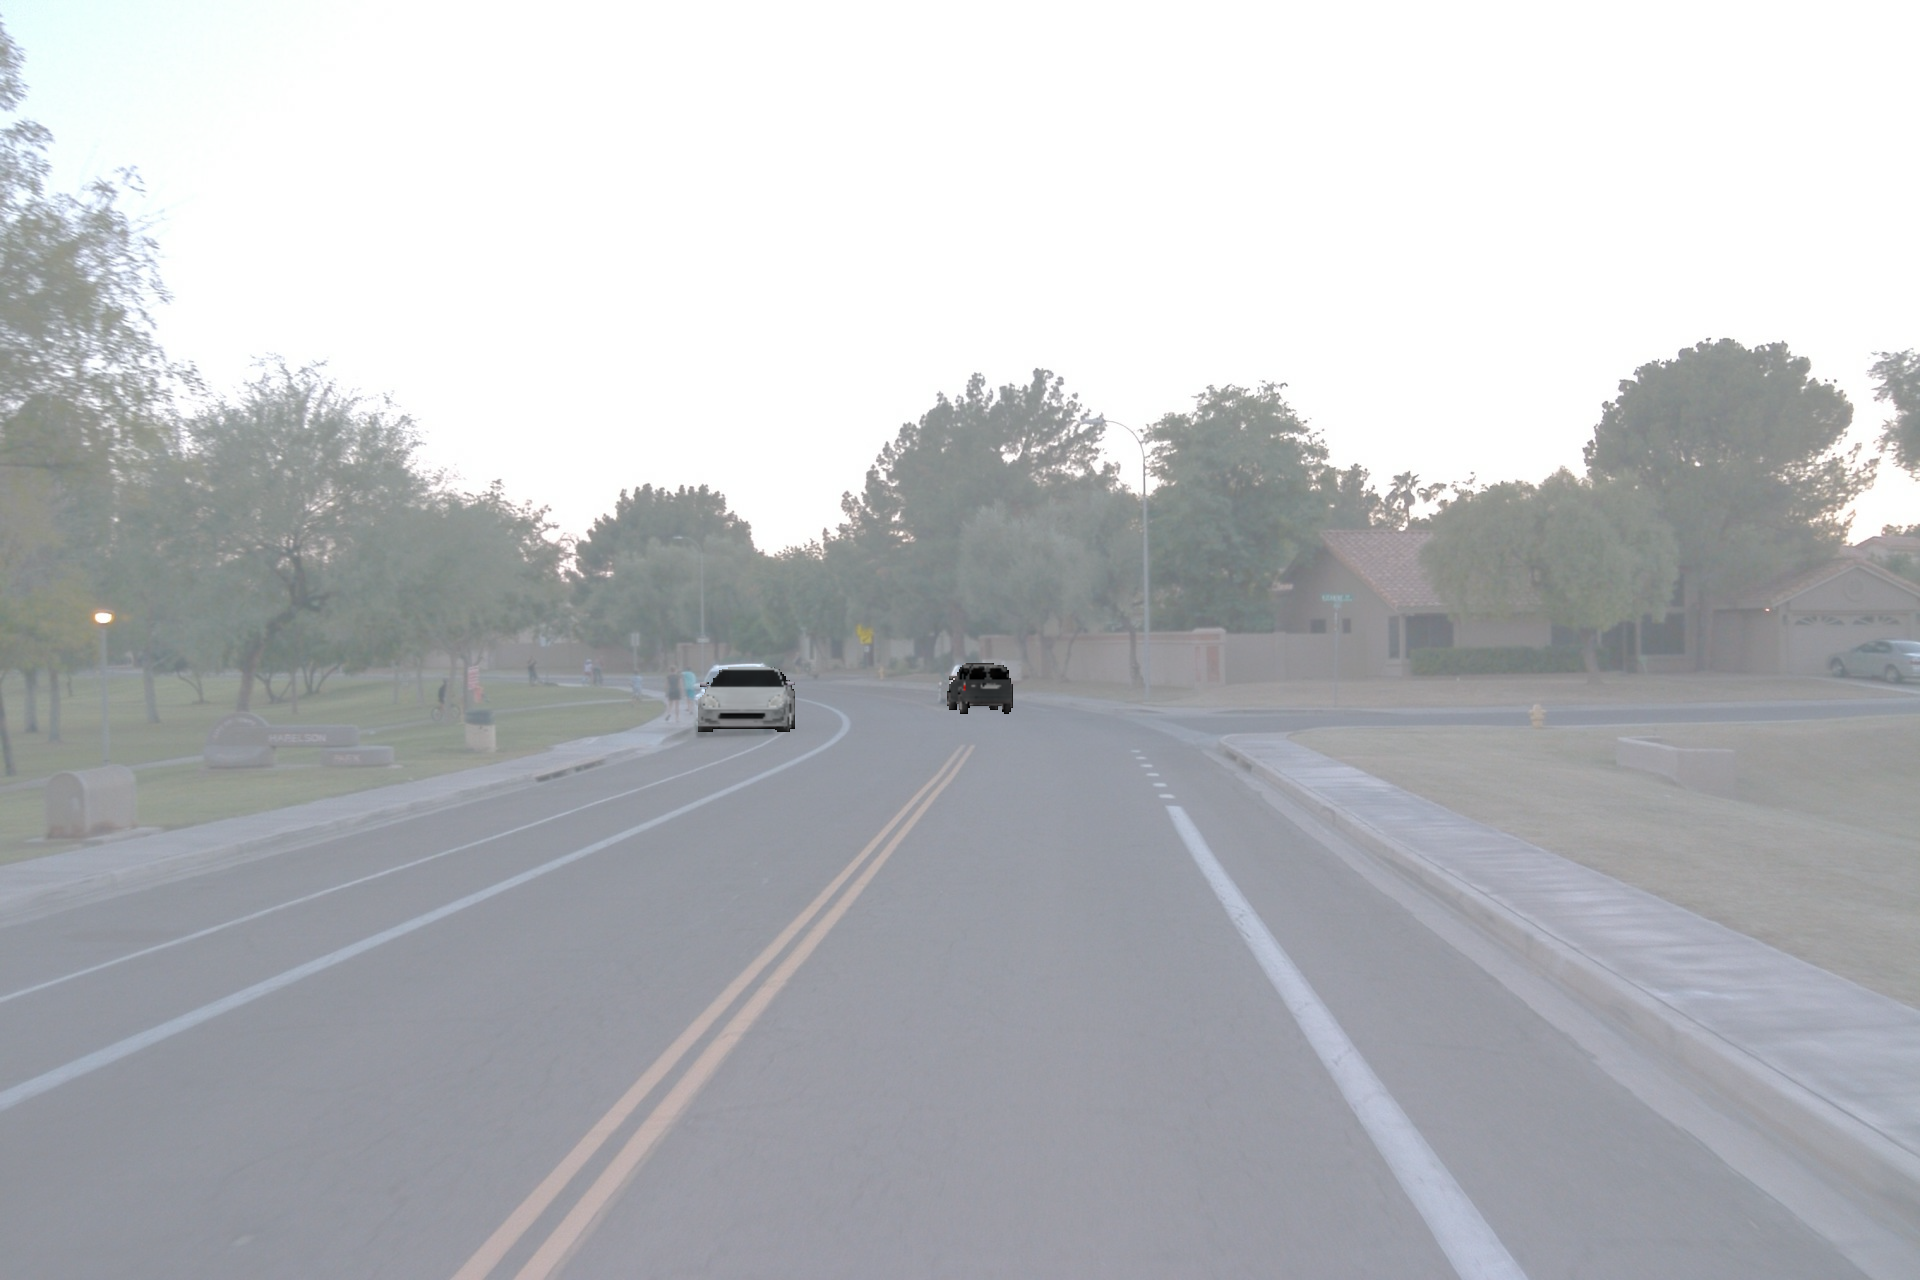
\includegraphics[width=.5\columnwidth, trim={22cm 16.68cm 30cm 18cm},clip]{fig/rebuttal_optimization/sched/82_60_shed.png} &
    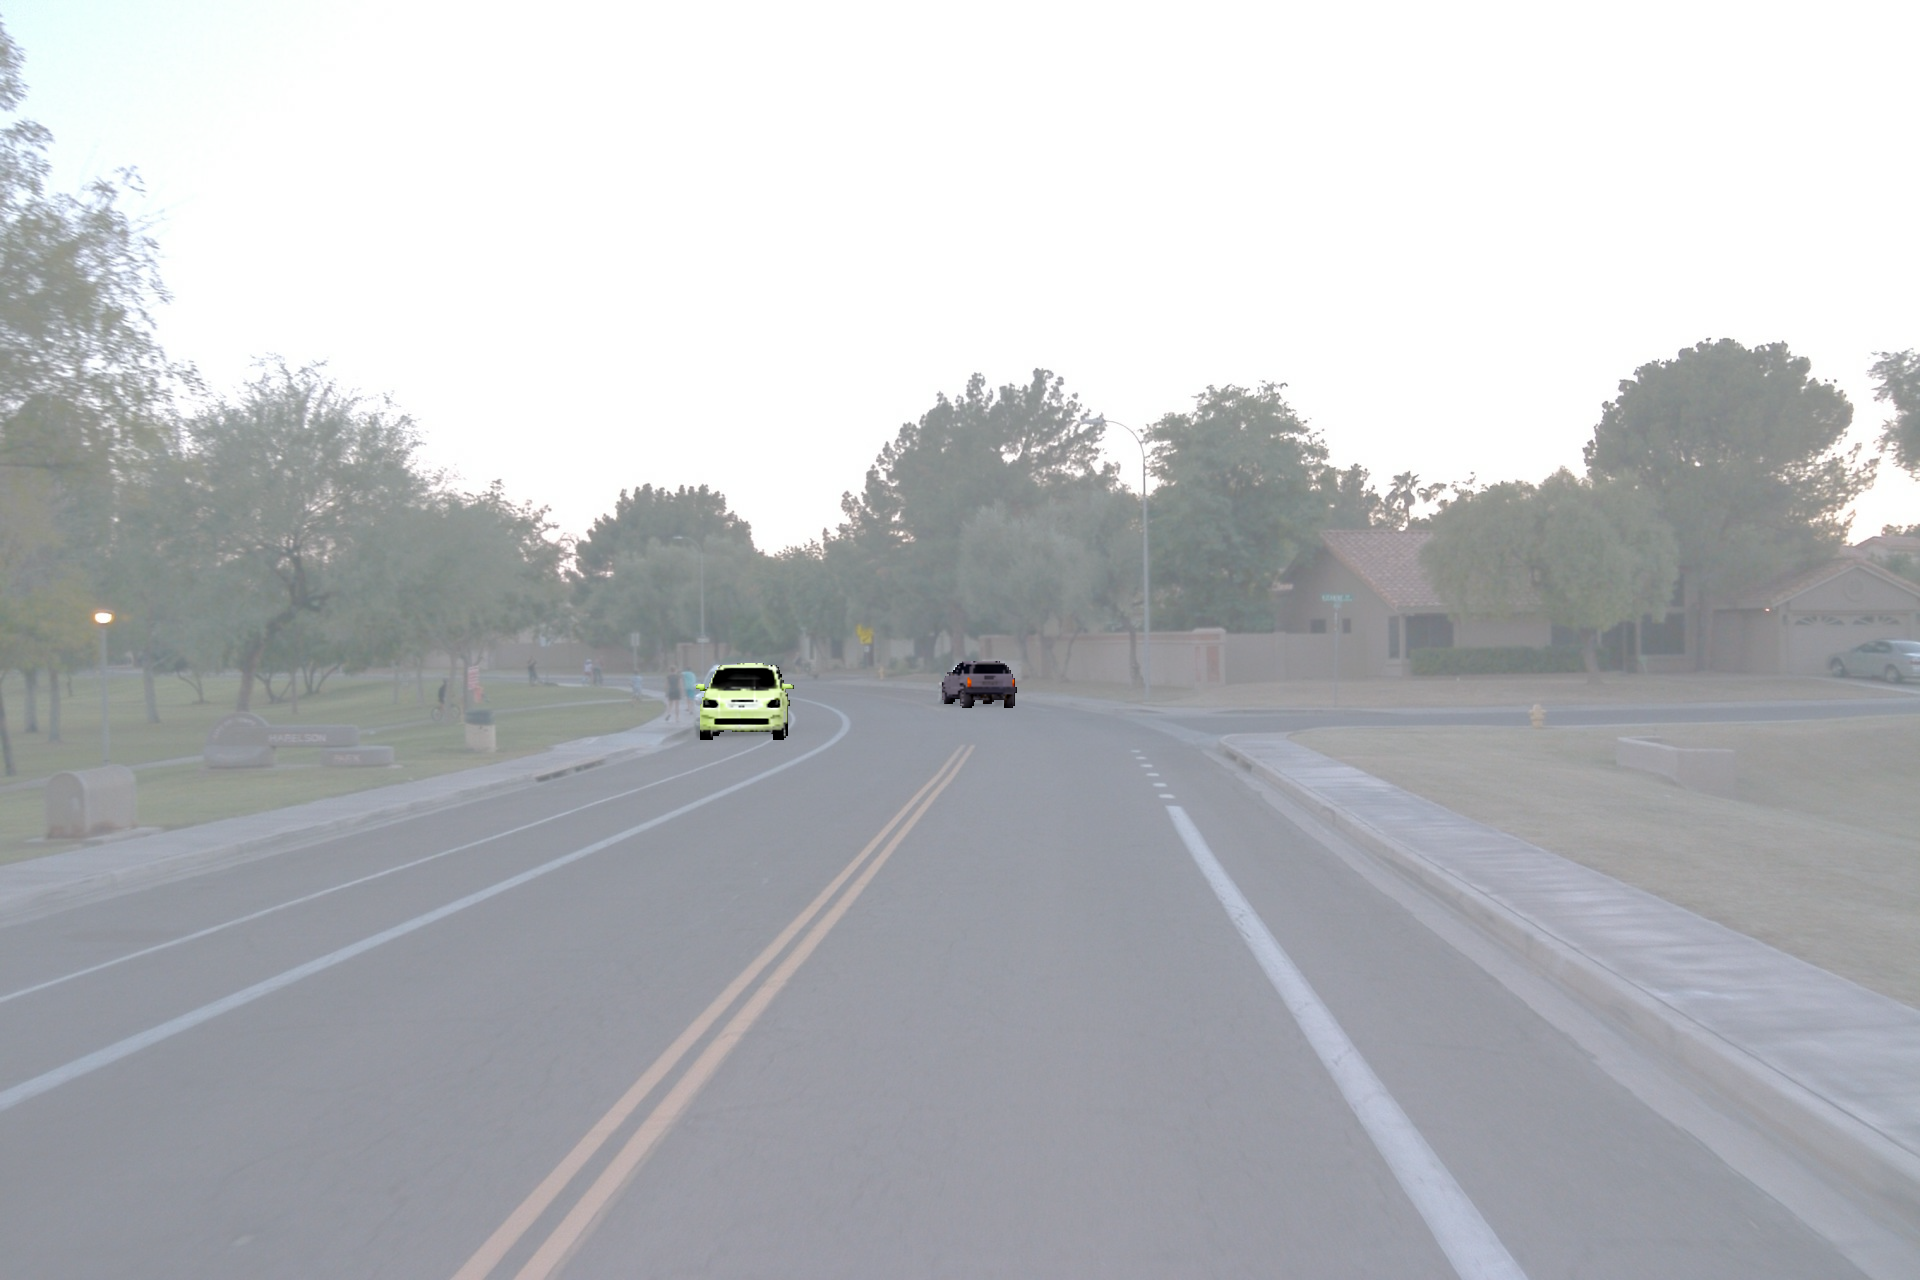
\includegraphics[width=.5\columnwidth, trim={22cm 16.68cm 30cm 18cm},clip]{fig/rebuttal_optimization/no_sched/82_60_no_shed.png}\\
    \multicolumn{3}{r}{\textit{Input frame is faded for visibility.}}
    \end{tabular}
}
    \vspace*{-6pt}
\label{fig:opt_scheduler}
\end{subtable}
\vspace*{-12pt}
\end{table}



% % \begin{table}[ht!]
\centering
\resizebox{0.95\linewidth}{!}{
\begin{tabular}{l|lll}
\hline
\hline
    Method (split)            & AMOTA $\uparrow$  & Recall $\uparrow$ & MOTA $\uparrow$   \\
    \hline
    AB3DMOT + CP (test) & 0.387             & 0.506             & 0.284             \\
    \hline
    Best Hyper-parameters (test)       & \textbf{0.402}    & \textbf{0.511}    & \textbf{0.320        }     \\
    \hline
    $w_{iou} = 1.4 $ (validation)   & 0.403             & 0.540             & 0.322               \\
    $w_{center} = 0.9$ (validation) & 0.417             & 0.514             & 0.332             \\
    $w_{embedd} = 0.4$ (validation) & 0.418             & 0.558             & 0.332             \\
    $\tau_{det} = 0.4$ (validation) & 0.397             & 0.567            & 0.326             \\
\hline
\hline
\end{tabular}
}
\caption{\textbf{Optimized Matching and Detection Confidence.} Parameters were optimized on the nuScenes \cite{caesar2020nuscenes} validation set. On the test split our best setting with $w_{iou} = 1.4$, $w_{center} = 0.9$, $w_{embbed} = 0.4$, $\tau_{det} = 0.4$ surpasses the performance of AB3DMOT \cite{weng2020AB3DMOT}, the only baseline not trained on the dataset. Results for other baselines are given in Tab. \ref{tab:nuScenes_results}. \todo{rewrite} }\label{tab:matching_ablations}
\vspace{-12pt}
\end{table}
% % \begin{table}[t]
\centering
\resizebox{0.9\linewidth}{!}{
\begin{tabular}{l|lll}
    \hline
    \hline
    Method & AMOTA $\uparrow$ & Recall $\uparrow$  & MOTA$\uparrow$  \\
    \hline
    No Schedule & 0.102 & 0.224 & 0.110  \\
    \hline
    $\mathcal{L}_{RGB}$ - Eq.~\ref{eq:loss_mse} & N/A  & N/A & N/A  \\
    $\mathcal{L}_{perceptual}$ - Eq.~\ref{eq:loss_lpips} & 0.100 & 0.251 & 0.101 \\
    $\mathcal{L}_{IR}$ - Eq.\ref{eq:loss_mse_lpips}  & 0.103 & 0.236   & 0.112 \\
    $\mathcal{L}_{IR}$ \& $\mathcal{L}_{embed}$ - Eq.\ref{eq:regularize}  & \textbf{0.112} & \textbf{0.264 } & \textbf{0.113} \\
\hline
\hline
\end{tabular}
}
\caption{\todo{(a) Make split figure} \textbf{Ablation Experiments on Optimization Schedule and Loss Components.} Ablations were run on a small subset of the nuScenes~\cite{caesar2020nuscenes} validation set.  $\mathcal{L}_{RGB}$ fails due to the optimizer fitting objects to the background instead, increasing the size of each object resulting in out of memory.}
\label{tab:optim_ablations}
\end{table}

% \begin{table}[t]
% % 1. Table
% \caption{\textbf{Ablation Experiments}}
% \vspace*{-12pt}
% \begin{subtable}[t]{0.485\linewidth}
% \centering
% \caption{\textbf{Optimization Schedule and Loss Components.} Ablations were run on a small subset of the nuScenes~\cite{caesar2020nuscenes} validation set.  $\mathcal{L}_{RGB}$ fails due to the optimizer fitting objects to the background instead, increasing the size of each object resulting in out of memory.}
% \vspace*{-6pt}
% \resizebox{0.98\textwidth}{!}{
% \begin{tabular}{l|lll}
%     \hline
%     \hline
%     Method & AMOTA $\uparrow$ & Recall $\uparrow$  & MOTA$\uparrow$  \\
%     \hline
%     $\mathcal{L}_{IR}$ \& $\mathcal{L}_{embed}$ - Eq.\ref{eq:regularize}  & \textbf{0.112} & \textbf{0.264 } & \textbf{0.113} \\
%     $\mathcal{L}_{IR}$ - Eq.\ref{eq:loss_mse_lpips}  & 0.103 & 0.236   & 0.112 \\
%     $\mathcal{L}_{perceptual}$ - Eq.~\ref{eq:loss_lpips} & 0.100 & 0.251 & 0.101 \\
%     $\mathcal{L}_{RGB}$ - Eq.~\ref{eq:loss_mse} & N/A  & N/A & N/A  \\
%     \hline
%     \underline{No Schedule} & 0.102 & 0.224 & 0.110  \\
% \hline
% \hline
% \end{tabular}
% }
% \label{tab:optim_ablations}
% \end{subtable}
% \hfill
% % 2. Table
% \begin{subtable}[t]{0.485\linewidth}
% \centering
% \caption{\textbf{Tracking Matching and Detection Confidence.} Parameters were optimized on the nuScenes \cite{caesar2020nuscenes} validation set. On the test split our best setting for $w_{iou}$, $w_{center}$, $w_{embbed}$, $\tau_{det}$ surpasses the performance of AB3DMOT \cite{weng2020AB3DMOT}, the only baseline not trained on the dataset. \todo{exchange with Figure 6}}
% \vspace*{-6pt}
% \resizebox{\linewidth}{!}{
% \begin{tabular}{l|lll}
%     \hline
%     \hline
%     Method (split) & AMOTA $\uparrow$ & Recall $\uparrow$ & MOTA $\uparrow$   \\
%     \hline
%     AB3DMOT + CP (test) & 0.387 & 0.506 & 0.284 \\
%     \hline
%     Best Hyper-param. (test) & \textbf{0.402} & \textbf{0.511} & \textbf{0.320} \\
%     \hline
%     $w_{iou} = 1.4 $ (val)   & 0.403             & 0.540             & 0.322 \\
%     $w_{center} = 0.9$ (val) & 0.417             & 0.514             & 0.332 \\
%     $w_{embedd} = 0.4$ (val) & 0.418             & 0.558             & 0.332 \\
%     $\tau_{det} = 0.4$ (val) & 0.397             & 0.567            & 0.326  \\
%     \hline
%     \hline
% \end{tabular}
% }
% \label{fig:matching_ablations}
% \end{subtable}
% \vspace*{-6pt}
% \end{table}